\documentclass[informe.tex]{subfiles}
\begin{document}

\section{Implementación (Constanza)}

Implemente su algoritmo \code{divide\_and\_conquer}, comparando sus respuestas con las de su
implementación de \code{brute\_force}.


\subsection{Código de implementación:}

\lstinputlisting[style=cpp, firstline=36, lastline=65]{../../src/divide_and_conquer.cpp}
\vspace{1em}

Más detalles de la implementación en el archivo del código (\code{src/divide\_and\_conquer.cpp}).


\subsection{Comparación:}
\begin{figure}[h] \centering 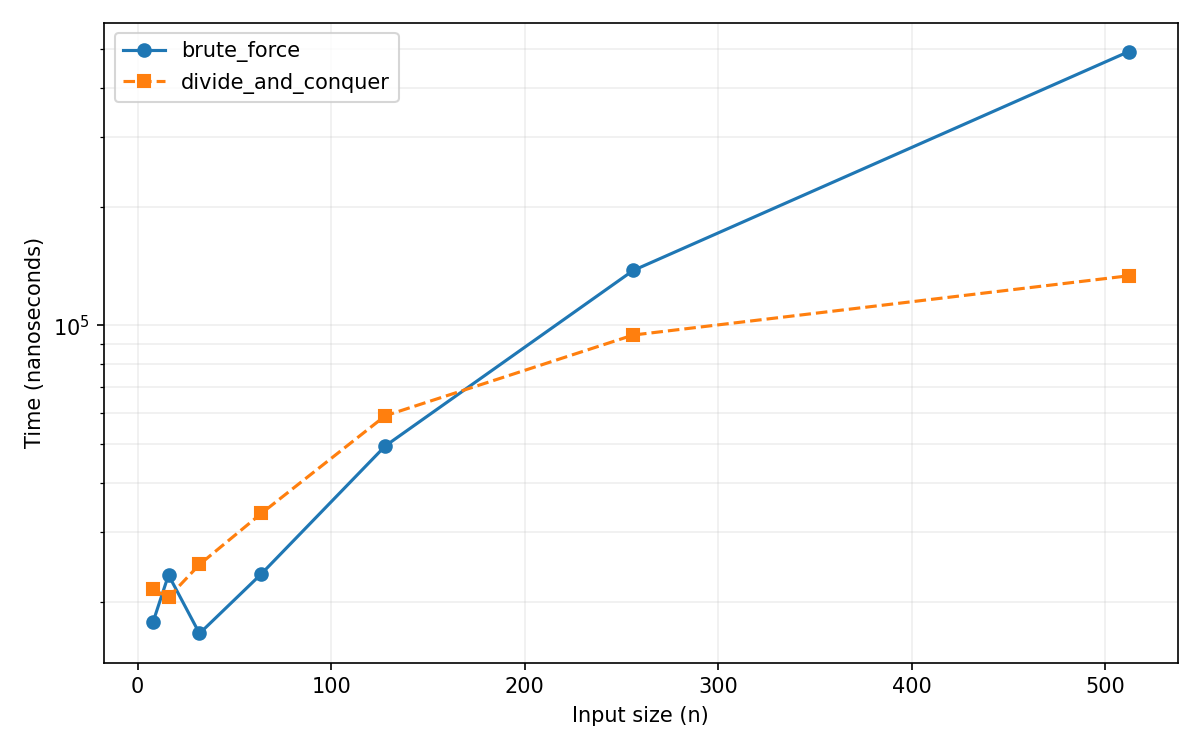
\includegraphics[width=0.8\textwidth]{img/plot_bf_dv.png}
	% \caption{gráfico comparando \code{brute\_force} y \code{divide\_and\_conquer}}
\end{figure}

\end{document}
